\documentclass[11pt]{article}

\usepackage{fancybox}



\usepackage{color}
\usepackage{url}
\usepackage[margin=1in]{geometry}


\renewcommand{\textfraction}{0.0}
\renewcommand{\topfraction}{1.0}
%\renewcommand{\textfloatsep}{5mm}

\usepackage{comment}
% Definitions of handy macros can go here
\usepackage{amsmath,amssymb,amsthm,bm,mathtools}
\usepackage{multirow}
\usepackage{natbib}
%\usepackage{dsfont,multirow,hyperref,setspace,natbib,enumerate}
\usepackage{dsfont,multirow,hyperref,setspace,enumerate}
\hypersetup{colorlinks,linkcolor={blue},citecolor={blue},urlcolor={red}}
\usepackage{algpseudocode,algorithm}
\algnewcommand\algorithmicinput{\textbf{Input:}}
\algnewcommand\algorithmicoutput{\textbf{Output:}}
\algnewcommand\INPUT{\item[\algorithmicinput]}
\algnewcommand\OUTPUT{\item[\algorithmicoutput]}

\mathtoolsset{showonlyrefs=true}



\theoremstyle{plain}
\newtheorem{thm}{Theorem}[section]
\newtheorem{lem}{Lemma}
\newtheorem{prop}{Proposition}
\newtheorem{pro}{Property}
\newtheorem{assumption}{Assumption}

\theoremstyle{definition}
\newtheorem{defn}{Definition}
\newtheorem{cor}{Corollary}
\newtheorem{example}{Example}
\newtheorem{rmk}{Remark}


\renewcommand{\thefigure}{{S\arabic{figure}}}%
\renewcommand{\thetable}{{S\arabic{table}}}%
\renewcommand{\figurename}{{Supplementary Figure}}
\renewcommand{\tablename}{{Supplementary Table}}
\setcounter{figure}{0}
\setcounter{table}{0}


\def\MLET{\hat \Theta_{\text{MLE}}}
\newcommand{\cmt}[1]{{\leavevmode\color{red}{#1}}}



\usepackage{dsfont}

\usepackage{multirow}

\DeclareMathOperator*{\minimize}{minimize}



\usepackage{mathtools}
\mathtoolsset{showonlyrefs}
\newcommand*{\KeepStyleUnderBrace}[1]{%f
  \mathop{%
    \mathchoice
    {\underbrace{\displaystyle#1}}%
    {\underbrace{\textstyle#1}}%
    {\underbrace{\scriptstyle#1}}%
    {\underbrace{\scriptscriptstyle#1}}%
  }\limits
}
\usepackage{xr}
\externaldocument{ordinalT}
\input macros.tex





\title{Some supplements}


%\author{%
%Chanwoo Lee \\
%University of Wisconsin -- Madison\\
 %\texttt{chanwoo.lee@wisc.edu} \\
%\And
%Miaoyan Wang \\
%University of Wisconsin -- Madison\\

%\texttt{miaoyan.wang@wisc.edu} \\
%}

\begin{document}


\begin{center}
\begin{spacing}{1.5}
\textbf{\Large Some supplements}
\end{spacing}
\end{center}
\section{Convexity}
\begin{thm}
\begin{align}
 \logl(\Theta, \mb)&=\sum_{\omega\in\Omega}\sum_{\ell\in[L]} \Big\{\mathds{1}_{\{y_\omega=\ell\}} \log \big[f(\theta_\omega+b_\ell)-  f(\theta_\omega+b_{\ell-1})\big]\Big\}, \text{ where } f(x) = \frac{e^x}{1+e^x}.
 \end{align}
is a concave function to $(\Theta,\mb)$
\end{thm}
\begin{proof}
It is enough to show that $\lambda(u,v) = \log \big[f(u)-  f(v)\big]$
is a concave function to $(u,v)$ where $u>v$. Because if $\lambda(u,v)$ is a concave function and $u,v$ are both linear functions of $(\Theta,\mb) $ such that $u = \ma_1^T(\Theta,\mb), v = \ma_2^T(\Theta,\mb)$, then $\lambda(u,v) = \lambda(\ma_1^T(\Theta,\mb),\ma_2^T(\Theta,\mb)))$ is a concave function to $(\Theta,\mb)$ by the definition of the convexity. With the fact that  $\logl(\Theta, \mb)$
can be written as the form of summations of $\lambda(u,v)$, we can conclude that $\logl(\Theta, \mb) $ is a concave function to $(\Theta,\mb)$ if we prove $\lambda(u,v)$ is concave. Write $\lambda(u,v) = \log\big[f(u)-f(v)\big]$ as $\log\big[\int\mathds{1}_{(u,v)}(x)f'(x)dx\big]$. Notice that  $\log\mathds{1}_{(u,v)}(x)$ is concave to $(u,v,x)$ and $\log f'(x)$ is concave to $x$ because $f'(x) = \frac{e^x}{(1+e^x)^2}$. Thus, $\log\mathds{1}_{(u,v)}(x)f'(x)$
is a concave function to $(u,v,x)$. Therefore, the $\lambda(u,v)$ is a concave function because the following lemma says that the integral of a log concave function with respect to some of its arguments is a log concave function of its remaining argument.
\end{proof}

\begin{lem}[Corollary 3.5 in~\cite{brascamp2002extensions}]
Let $F(x,y):\mathbb{R}^{m+n}\rightarrow \mathbb{R}$ be an integrable function where $x\in \mathbb{R}^{m},y\in \mathbb{R}^n$. Let $$G(x) = \int_{\mathbb{R}^n}F(x,y)dy.$$ If $F(x,y)$ is a log concave function to (x,y), then $G(x)$ is a log concave function.
\end{lem}

\section{Property of an estimator}

\begin{pro}
$y^{(\text{Median})}_\omega$ minimizes $R(y) = \mathbb{E}_{\hat{\theta}_\omega,\hat{\mb}}|y_\omega-y|$.
\end{pro}
\begin{proof}
We can write $R(y) = \sum_{\ell\in[L]}|\ell-y|\hat f_\ell$ where $\hat f_\ell = f_\ell(\hat{\theta}_\omega,\hat\mb)$. Let us denote $\mu = y^{(\text{Median})}_\omega$. Then,
\begin{align*}
  R(y)&=
  \begin{cases}
  \big[- (\hat f_1 \cdots +\hat f_L)\big]y + \big[(L\hat f_L+\cdots +1\hat f_1)\big],& \text{if $y\in(-\infty,1]$},\\
  \big[\hat f_1 - (\hat f_2 \cdots +\hat f_L)\big]y + \big[(L\hat f_L+\cdots +2\hat f_2) -1\hat f_1\big],& \text{if $y\in(1,2]$},\\
  \vdots & \vdots\\
  \big[(\hat f_1 +\cdots + \hat f_{\mu-1}) - (\hat f_{\mu} \cdots +\hat f_L)\big]y + \big[(L\hat f_L+\cdots +\mu\hat f_\mu) -((\mu-1)\hat f_{\mu-1}+\cdots+1\hat f_1)\big],& \text{if $y\in(\mu-1, \mu]$},\\
  \big[(\hat f_1 +\cdots + \hat f_{\mu}) - (\hat f_{\mu+1} \cdots +\hat f_L)\big]y + \big[(L\hat f_L+\cdots +(\mu+1)\hat f_{\mu+1}) -(\mu\hat f_\mu+\cdots+1\hat f_1)\big],& \text{if $y\in(\mu, \mu+1]$} \\
  \vdots  &\vdots\\
  \big[(\hat f_1 +\cdots + \hat f_{L-1}) - \hat f_L)\big]y + \big[(L\hat f_L -((L-1)\hat f_{L-1}+\cdots+1\hat f_1)\big],& \text{if $y\in(L-1, L]$},\\
  \big[(\hat f_1 +\cdots + \hat f_{L})\big]y + \big[(L\hat f_L+\cdots+1\hat f_1)\big],& \text{if $y\in(L, \infty]$}.\\
  \end{cases}
\end{align*}
Based on the above formula, we can find out that $R(y)$ is minimized when $y = \mu$ because $ (\hat f_1 +\cdots + \hat f_{\mu-1}) - (\hat f_{\mu} \cdots +\hat f_L)<0 $ and $ (\hat f_1 +\cdots + \hat f_{\mu}) - (\hat f_{\mu+1} \cdots +\hat f_L)>0$ by the definition of $\mu$.
\end{proof}

\section{Theorems in the case when the cut points is unknown}
When the cut points $\mb$ is unknown, we estimate $(\hat\Theta,\hat\mb)$ by alternately fixing each factor and proceed until each factor does not change from each update. We have the following relationship between $\hat\Theta$ and $\hat\mb$
\begin{equation}
  \begin{aligned}
    \hat\Theta = \argmax_{\Theta\in \mathcal{P}} \logl (\Theta|\hat\mb)\quad \text{ and }\quad \hat\mb = \argmax_{\mb\in \mathcal{B}}\logl(\mb|\hat\Theta).
  \end{aligned}
\end{equation}
We assess the estimation accuracy using the mean squared error (MSE):
$$\text{MSE}(\hat\Theta,\hat\mb) = \frac{1}{\prod_k d_k}\FnormSize{}{(\hat\Theta,\hat\mb)-(\Theta^{\text{true}},\mb^{\text{true}})}. $$
We show that $\frac{1}{\prod_k d_k}\FnormSize{}{(\hat\Theta,\hat\mb)-(\hat\Theta,\mb^{\text{true}})} $ is bounded by $o(\frac{1}{\prod_k d_k})$ with high probability so that $$ \frac{1}{\prod_k d_k}\FnormSize{}{(\hat\Theta,\hat\mb)-(\Theta^{\text{true}},\mb^{\text{true}})} \leq \frac{1}{\prod_k d_k}\FnormSize{}{\hat\Theta-\Theta^{\text{true}}} + o(\frac{1}{\prod_k d_k}).$$
Therefore, we can utilize Theorem 4.1 to establish the upper bound for the proposed $(\hat\Theta,\hat\mb).$
We define a few key quantities that will be used in the proof.
\begin{align}
 U_\alpha &= \max_{\ell\in[L-1],|\theta|\leq \alpha} \max(\frac{\dot{f}(\theta+b_\ell)}{f(\theta+b_\ell)-f(
\theta+b_{\ell-1})},\frac{\dot{f}(\theta+b_\ell)}{f(\theta+b_{\ell+1})-f(
\theta+b_{\ell})})\\
L_\alpha & = \min_{\ell\in[L-1],|\theta|\leq \alpha} \min(-\frac{\ddot{f}(\theta+b_\ell)[f(\theta+b_\ell)-f(\theta+b_{\ell-1})]-\dot{f}(\theta+b_\ell)[\dot{f}(\theta+b_\ell)-\dot{f}(\theta+b_{\ell-1})]}{[f(\theta+b_\ell)-f(\theta+b_{\ell-1})]^2},
\\ &\hspace{1in}\qquad\frac{\ddot{f}(\theta+b_\ell)[f(\theta+b_{\ell+1})-f(\theta+b_{\ell})]-\dot{f}(\theta+b_\ell)[\dot{f}(\theta+b_{\ell+1})-\dot{f}(\theta+b_{\ell})]}{[f(\theta+b_{\ell+1})-f(\theta+b_{\ell})]^2})
\end{align}
We can see $U_\alpha>0$ and $L_\alpha>0$ from the assumption. Especially when $f(x) = \frac{1}{1+e^{-x}}$ , we have $$L_\alpha = \min_{\ell\in[L-1],|\Theta|\leq\alpha}\min\bigg(\frac{e^{\theta+b_\ell} (e^{\theta+b_\ell} - e^{\theta+b_{\ell-1}})^2}{(e^{\theta+b_\ell} + 1)^4 (e^{\theta+b_{\ell-1}} + 1)^2},\frac{e^{\theta+b_\ell} (e^{\theta+b_{\ell+1}} - e^{\theta+b_\ell})^2}{(e^{\theta+b_{\ell+1}} + 1)^2 (e^{\theta+b_\ell} + 1)^4}\bigg).$$
\begin{thm}
  From the same setting in Theorem 4.1 except the knowledge of $\mb$, with very high probability, the estimator satisfies
  \begin{equation}
    \frac{1}{\prod_k d_k}\FnormSize{}{(\hat\Theta,\hat\mb)-(\hat\Theta,\mb^{\text{true}})} = o(\frac{1}{\prod_k d_k}).
  \end{equation}
\end{thm}

\begin{proof}
It follows from the expression of $\logl(\Theta,\mb)$ that
\begin{align}\label{eq:property}
{\partial \flogl\over \partial \beta_\ell}&=\sum_{\omega\in\Omega}\bigg[\mathds{1}_{\{y_{\omega}=\ell\}}
\frac{\dot{f}(\theta_\omega+b_\ell)}{f(\theta_\omega+b_\ell)-f(
\theta_\omega+b_{\ell-1})}-\mathds{1}_{\{y_{\omega}=\ell+1\}}
\frac{\dot{f}(\theta_\omega+b_\ell)}{f(\theta_\omega+b_{\ell+1})-f(\theta_\omega+b_{\ell})}\bigg],\notag\\
{\partial^2 \flogl\over \partial b_\ell^2}&=\sum_{\omega\in\Omega}\bigg[\mathds{1}_{\{y_\omega=\ell\}}\frac{\ddot{f}(\theta_\omega+b_\ell)[f(\theta_\omega+b_\ell)-f(\theta_\omega+b_{\ell-1})]-\dot{f}(\theta_\omega+b_\ell)^2}{[f(\theta_\omega+b_\ell)-f(\theta_\omega+b_{\ell-1})]^2}\\
&\hspace{.6in}-\mathds{1}_{\{y_\omega=\ell+1\}}\frac{\ddot{f}(\theta_\omega+b_\ell)[f(\theta_\omega+b_{\ell+1})-f(\theta_\omega+b_{\ell})]+\dot{f}(\theta_\omega+b_\ell)^2}{[f(\theta_\omega+b_{\ell+1})-f(\theta_\omega+b_{\ell})]^2}\bigg] \text{ for } \ell \in [L-1],\\
{\partial^2 \flogl\over \partial b_\ell \partial b_{\ell+1}}&=\sum_{\omega\in\Omega}\mathds{1}_{\{y_\omega=\ell+1\}}\frac{\dot{f}(\theta_\omega+b_\ell)\dot{f}(\theta_\omega+b_{\ell+1})}{[f(\theta_\omega+b_{\ell+1})-f(\theta_\omega+b_\ell)]^2} \text{ for } \ell \in [L-2] \text{ and } {\partial^2 \flogl\over \partial b_i \partial b_j} = 0 \text{ if } |i-j|>1.
\end{align}
Therefore, all entries in $\frac{1}{\prod_k d_k}\fploglb$ are upper bounded $U>0$, and  $\frac{1}{\prod_k d_k}\fpploglb$ is a tridiagonal matrix.




By the second-order Taylor's expansion of $\flogl(\mb|\hat\Theta)$ around $\mb^{\text{true}}$, we obtain
\begin{equation}\label{eq:taylor}
\flogl(\hat\mb|\hat\Theta)=\flogl(\mb^{\text{true}}|\hat\Theta)+(\trueb-\hat\mb)^T\fploglb(\trueb)+ (\trueb-\hat\mb)^T\fpploglb(\check\mb)(\trueb-\hat\mb),
\end{equation}
$\check\mb=\gamma\trueb+(1-\gamma)\hat\mb$ for some $\gamma\in[0,1]$, and $\fpploglb(\check\mb)$ denotes the $(L-1)$-by-$(L-1)$ Hession matrix evaluated at $\check\mb$.

We first bound the linear term in~\eqref{eq:taylor}. Note that, by Cauchy-Schwartz inequality,
\begin{equation}\label{eq:linear}
(\trueb-\hat\mb)^T\fploglb(\trueb)\leq \|\trueb-\hat\mb\|\|\fploglb(\trueb)\|
\leq \|\trueb-\hat\mb\|U_\alpha\sqrt{L} \prod_k d_k .\end{equation}
The last inequality is followed by
\[
{\partial \tL_\tY\over \partial b_\ell}\Big|_{\mb=\trueb} \leq U_\alpha \;\; \textrm{ for all } \; l\in [L-1].
\]

We next bound the quadratic term in \eqref{eq:taylor}. Note that
\begin{align}\label{eq:quadratic}
 &(\trueb-\hat\mb))^T \fpploglb(\check{\mb})(\trueb-\hat\mb)\\
 &=\sum_{\ell\in [L-1]} \left( {\partial^2\tL_{\tY}\over \partial b^2_\ell} \Big|_{\mb=\check\mb} \right)(\hat b_\ell-b_{{\text{true}},\ell})^2 + 2\sum_{\ell\in[L-1]-\{1\}}\left( {\partial^2\tL_{\tY}\over \partial b_\ell \partial b_{\ell-1}} \Big|_{\mb=\check\mb} \right)(\hat b_\ell-b_{{\text{true}},\ell})(\hat b_{\ell-1}-b_{{\text{true}},\ell-1}) \nonumber \\
&\leq \sum_{\ell\in [L-1]} \left( {\partial^2\tL_{\tY}\over \partial b^2_\ell} \Big|_{\mb=\check\mb} \right)(\hat b_\ell-b_{{\text{true}},\ell})^2 + \sum_{\ell\in[L-1]-\{1\}}\left( {\partial^2\tL_{\tY}\over \partial b_\ell \partial b_{\ell-1}} \Big|_{\mb=\check\mb} \right)\big[(\hat b_\ell-b_{{\text{true}},\ell})^2 +(\hat b_{\ell-1}-b_{{\text{true}},\ell-1})^2\big] \nonumber \\
&=\left( {\partial^2\tL_{\tY}\over \partial b^2_1}+{\partial^2\tL_{\tY}\over \partial b_1 \partial b_2 }\Big|_{\mb=\check\mb} \right)(\hat b_1-b_{{\text{true}},1})^2+\left( {\partial^2\tL_{\tY}\over \partial b^2_{L-1}}+{\partial^2\tL_{\tY}\over \partial b_{L-2} \partial b_{L-1} }\Big|_{\mb=\check\mb} \right)(\hat b_{L-1}-b_{{\text{true}},L-1})^2  \\
&+\sum_{\ell\in[L-2]-\{1\}}\left( {\partial^2\tL_{\tY}\over \partial b^2_\ell}+{\partial^2\tL_{\tY}\over \partial b_\ell \partial b_{\ell-1}}+{\partial^2\tL_{\tY}\over \partial b_{\ell+1} \partial b_{\ell}} \Big|_{\mb=\check\mb} \right)(\hat b_\ell-b_{{\text{true}},\ell})^2     \\
&\leq - L_\alpha\prod_k d_k \sum_{\ell \in [L-1]}(\hat b_\ell-b_{\text{true},\ell})^2 \nonumber \\
&=-L_\alpha\prod_k d_k\FnormSize{}{\hat\mb-\trueb}^2,
\end{align}
Therefore, combining~\eqref{eq:taylor} and the above linear term and quadratic term results, we have that,
\[
\tL_\tY(\hat\mb|\hat\Theta)\leq \tL_{\tY}(\trueb|\hat\Theta)+U_\alpha\sqrt{L}\prod_k d_k\FnormSize{}{\hat\mb-\trueb} -\frac{L_\alpha}{2}\prod_k d_k \FnormSize{}{\hat\mb-\trueb}^2 .
\]

Since $\hat \mb=\arg\max_{\mb\in\tB}\tL_\tY(\mb|\hat\Theta)$, $\tL_\tY(\hat\mb|\hat\Theta))-\tL_\tY(\trueb|\hat\Theta)\geq 0$, which gives
\[
U_\alpha\sqrt{L}\FnormSize{}{\hat\mb-\trueb} -\frac{L_\alpha}{2} \FnormSize{}{\hat\mb-\trueb}^2\geq 0.
\]
Henceforth,
\[
\FnormSize{}{\hat\mb-\trueb}\leq \frac{2U_\alpha \sqrt{L}}{L_\alpha}.
\]
Finally, this complete the proof.
\begin{equation}
  \frac{1}{\prod_k d_k}\FnormSize{}{(\hat\Theta,\hat\mb)-(\hat\Theta,\mb^{\text{true}})} =\frac{1}{\prod_k d_k}\FnormSize{}{\hat\mb-\trueb}
  = o(\frac{1}{\prod_k d_k}).
\end{equation}.

\section{Brain data clustering}

\begin{table}[]
\begin{tabular}{|c|c|c|c|c|c|c|}
\hline
Group       & \multicolumn{3}{c|}{\#1}                                                  & \multicolumn{3}{c|}{\#2}                                      \\ \hline
Brain nodes & \multicolumn{3}{l|}{\begin{tabular}[c]{@{}l@{}}"RMF\_L","Fpole\_L","Insula\_L",\\ "SupF\_L","CaudMF\_L",\\ "parsTriangularis\_L","parsOpercularis\_L",\\ "preCentral\_L","Tpole\_L","SupT\_L",\\ "SupT\_L","postCentral\_L", "SupP\_L",\\ "IP\_L","LO\_L","MOF\_L","SupF\_L",\\ "IsthmusC\_L","Precuneus\_L",\\ "Cuneus\_L","paraHippo\_L",\\ "Lingual\_L","SupT\_L","LO\_L"\end{tabular}} & \multicolumn{3}{l|}{\begin{tabular}[c]{@{}l@{}}"RMF\_R","Fpole\_R","Insula\_R",\\ "SupF\_R", "CaudMF\_R",\\ "parsTriangularis\_R" ,"parsOpercularis\_R",\\ "preCentral\_R", "Tpole\_R","SupT\_R",\\ "SupT\_R","postCentral\_R","SupP\_R",\\ "IP\_R","LO\_R","MOF\_R", "SupF\_R",\\ "IsthmusC\_R","Precuneus\_R",\\ "Cuneus\_R","paraHippo\_R",\\ "Lingual\_R","SupT\_R","LO\_R"\end{tabular}} \\ \hline
Group       & \#3    & \#4    & \#5   & \#6  & \#7 & \#8
\\ \hline
Brain nodes & \begin{tabular}[c]{@{}c@{}}"SupraM\_L" \\ "SupraM\_L" \\ "SupraM\_L" \\ "SupraM\_L"\end{tabular}                                      & \begin{tabular}[c]{@{}c@{}}"SupraM\_R" \\ "SupraM\_R" \\ "SupraM\_R" \\ "SupraM\_R"\end{tabular}                                      & \begin{tabular}[c]{@{}c@{}}"IT\_L" \\ "IT\_L" \\ "IT\_L"\end{tabular}                                      & \begin{tabular}[c]{@{}c@{}}"IT\_R" \\ "IT\_R" \\ "IT\_R"\end{tabular}                                                          & \begin{tabular}[c]{@{}c@{}}"MT\_L" \\ "MT\_L" \\ "MT\_L"\end{tabular}                                                         & \begin{tabular}[c]{@{}c@{}}"MT\_R" \\ "MT\_R"\\ "MT\_R"\end{tabular}                                                         \\ \hline
\end{tabular}
\end{table}
\begin{figure}[H]
  \centering
 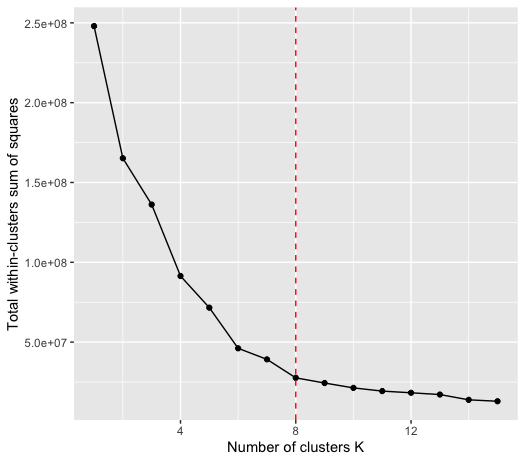
\includegraphics[width = 0.45\textwidth]{elbowmethod.png}

  \label{figure:cluster graph}
  \caption{Brain cluster graph}
\end{figure}


\begin{figure}[H]
  \centering
 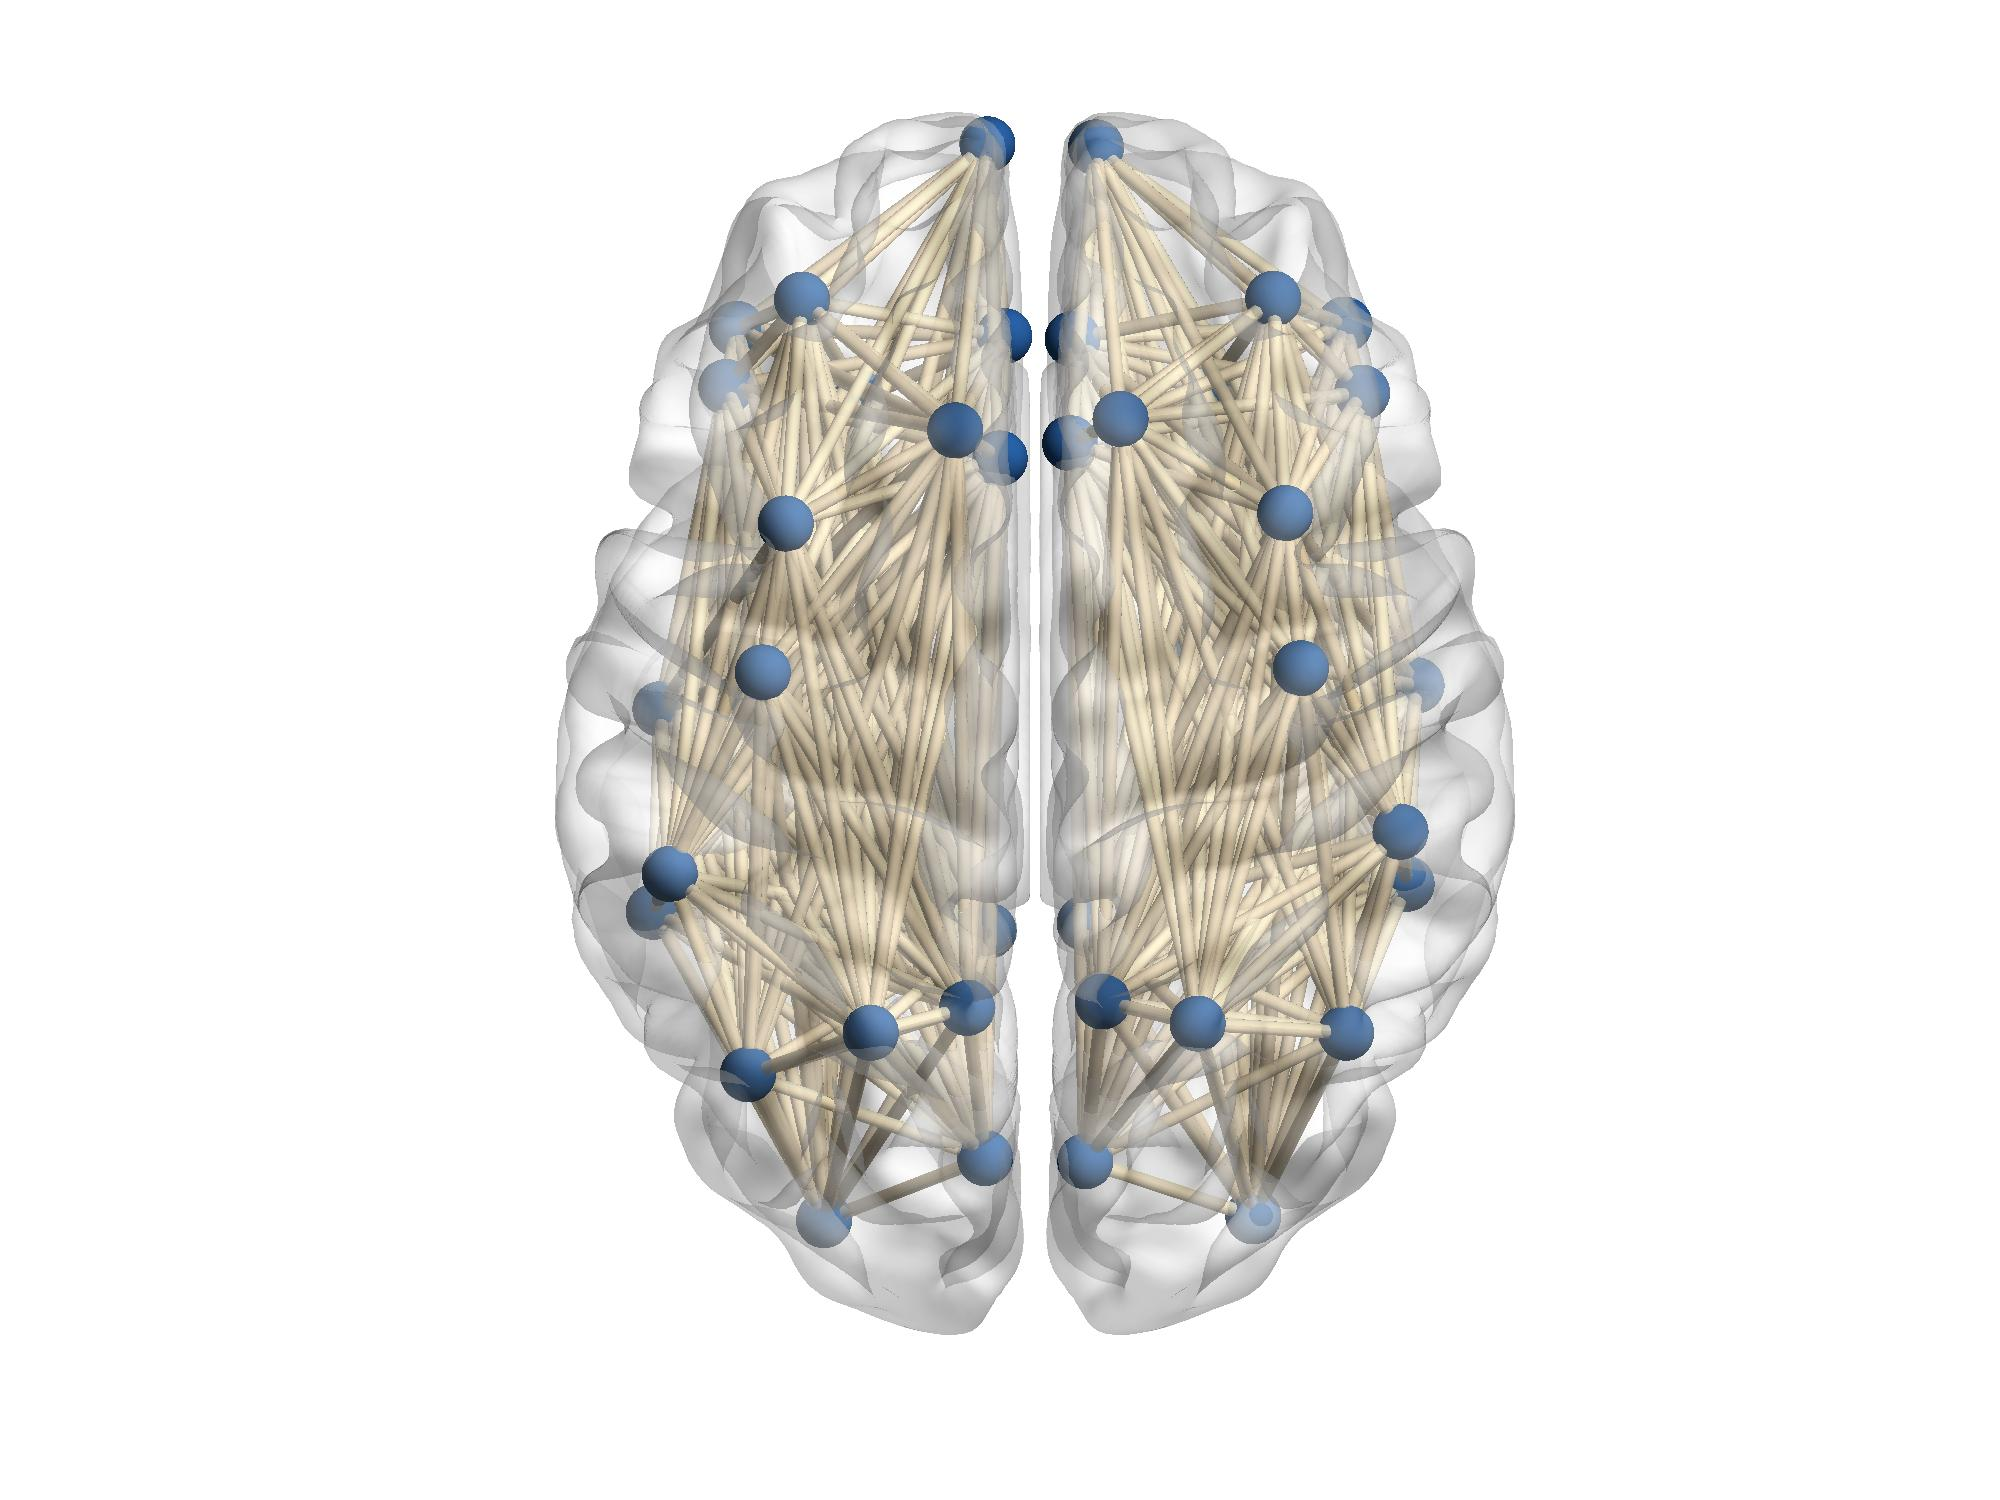
\includegraphics[width = 0.45\textwidth]{brain1.jpg}
 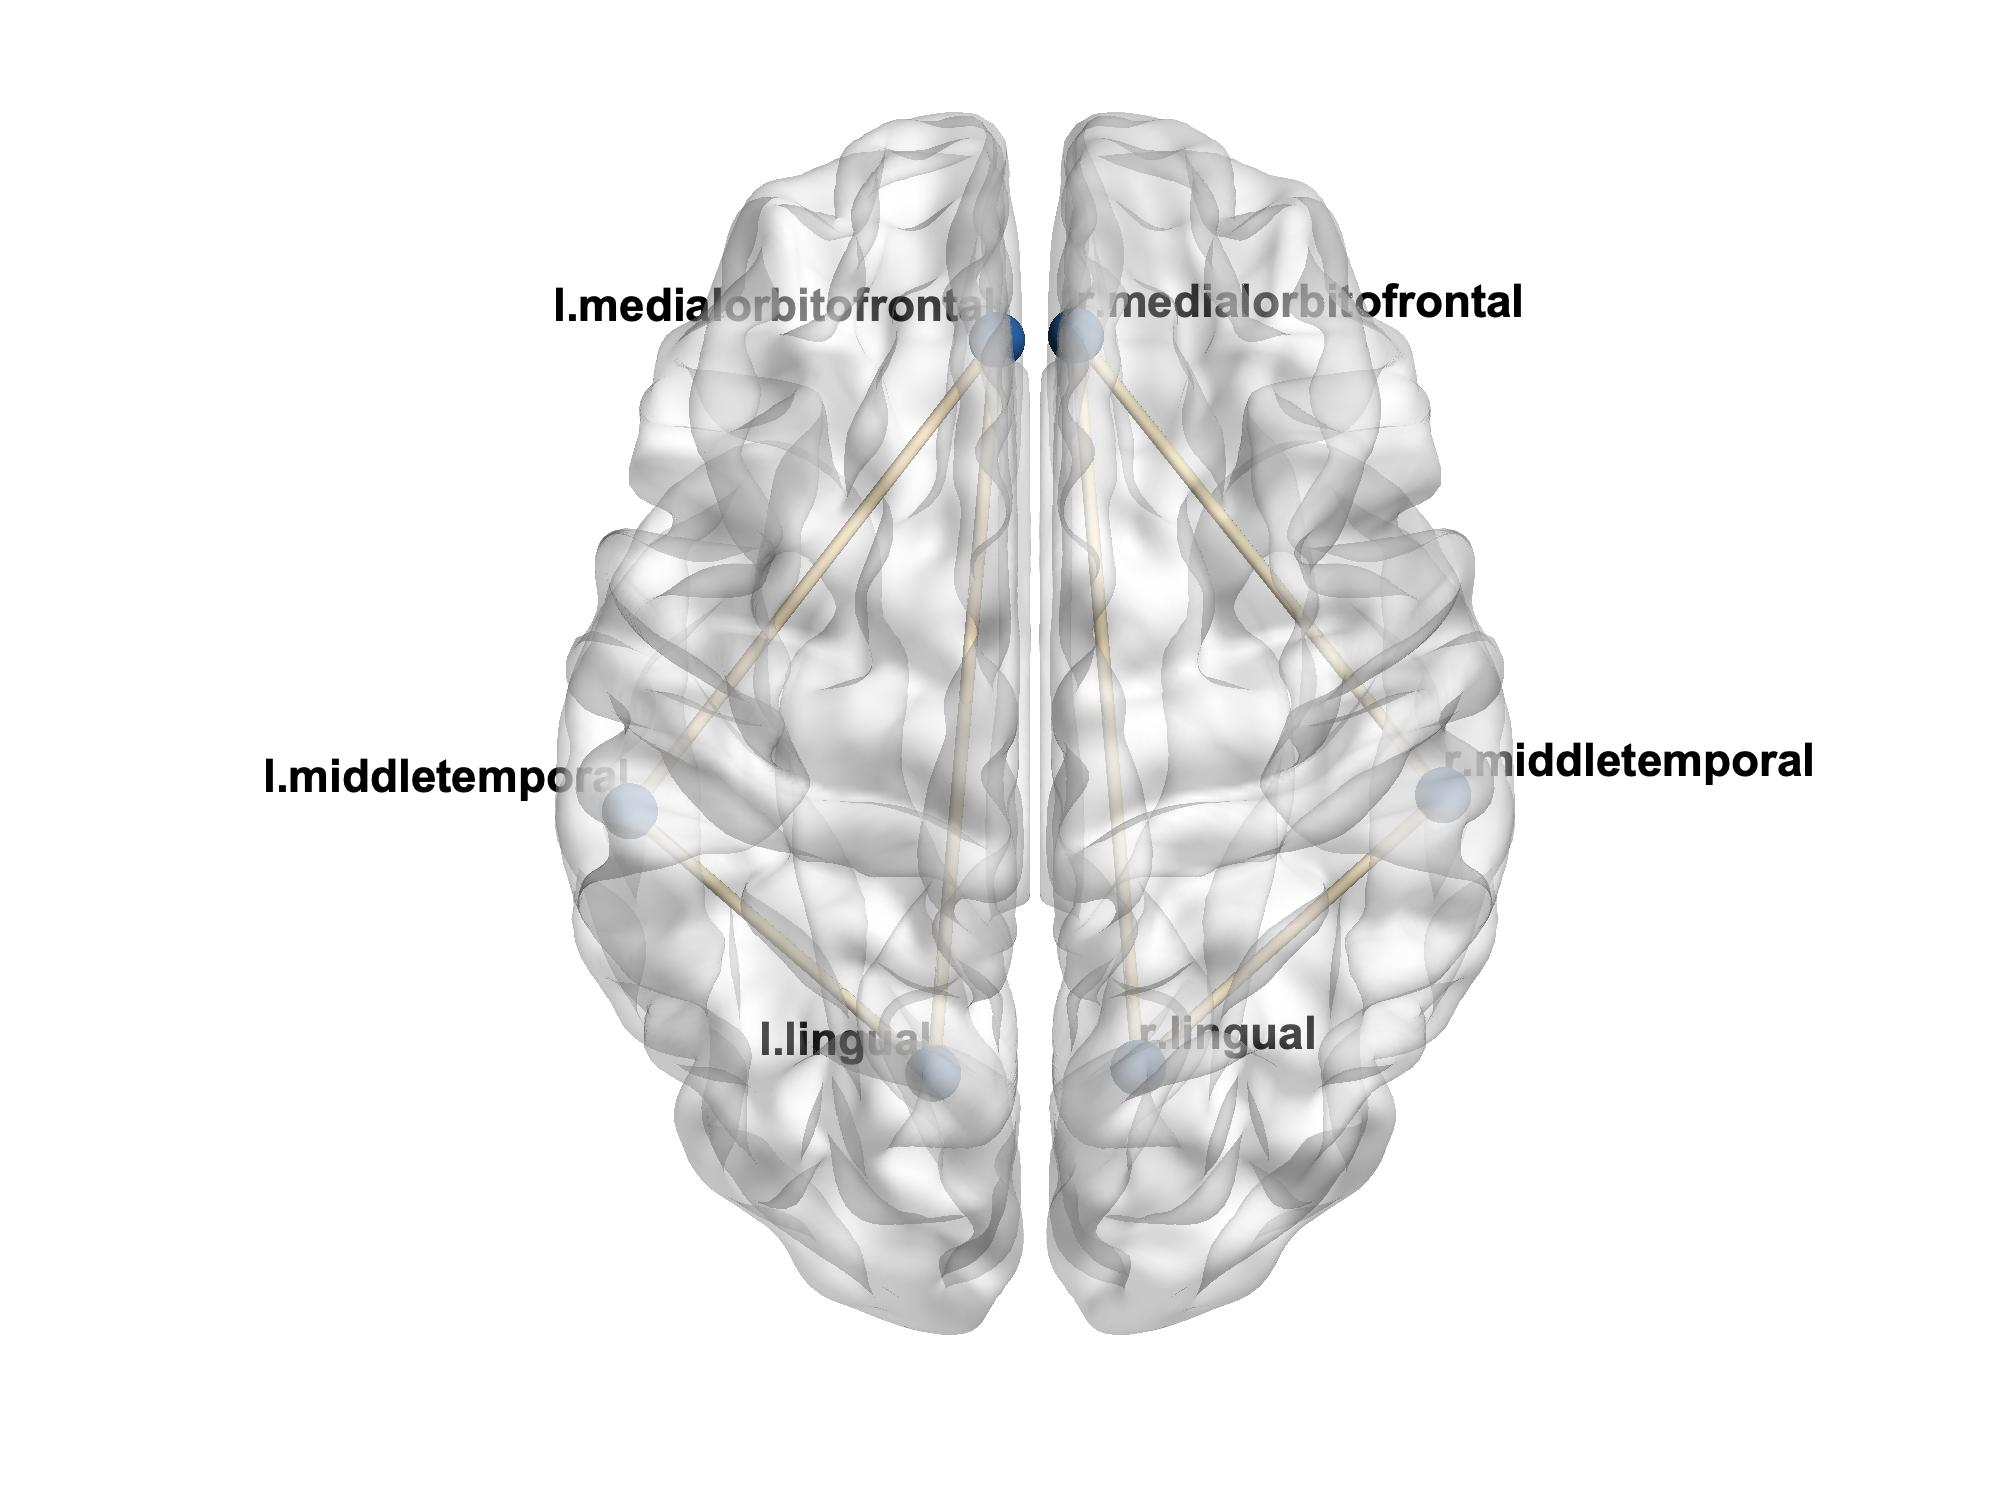
\includegraphics[width = 0.45\textwidth]{brain2.jpg}
 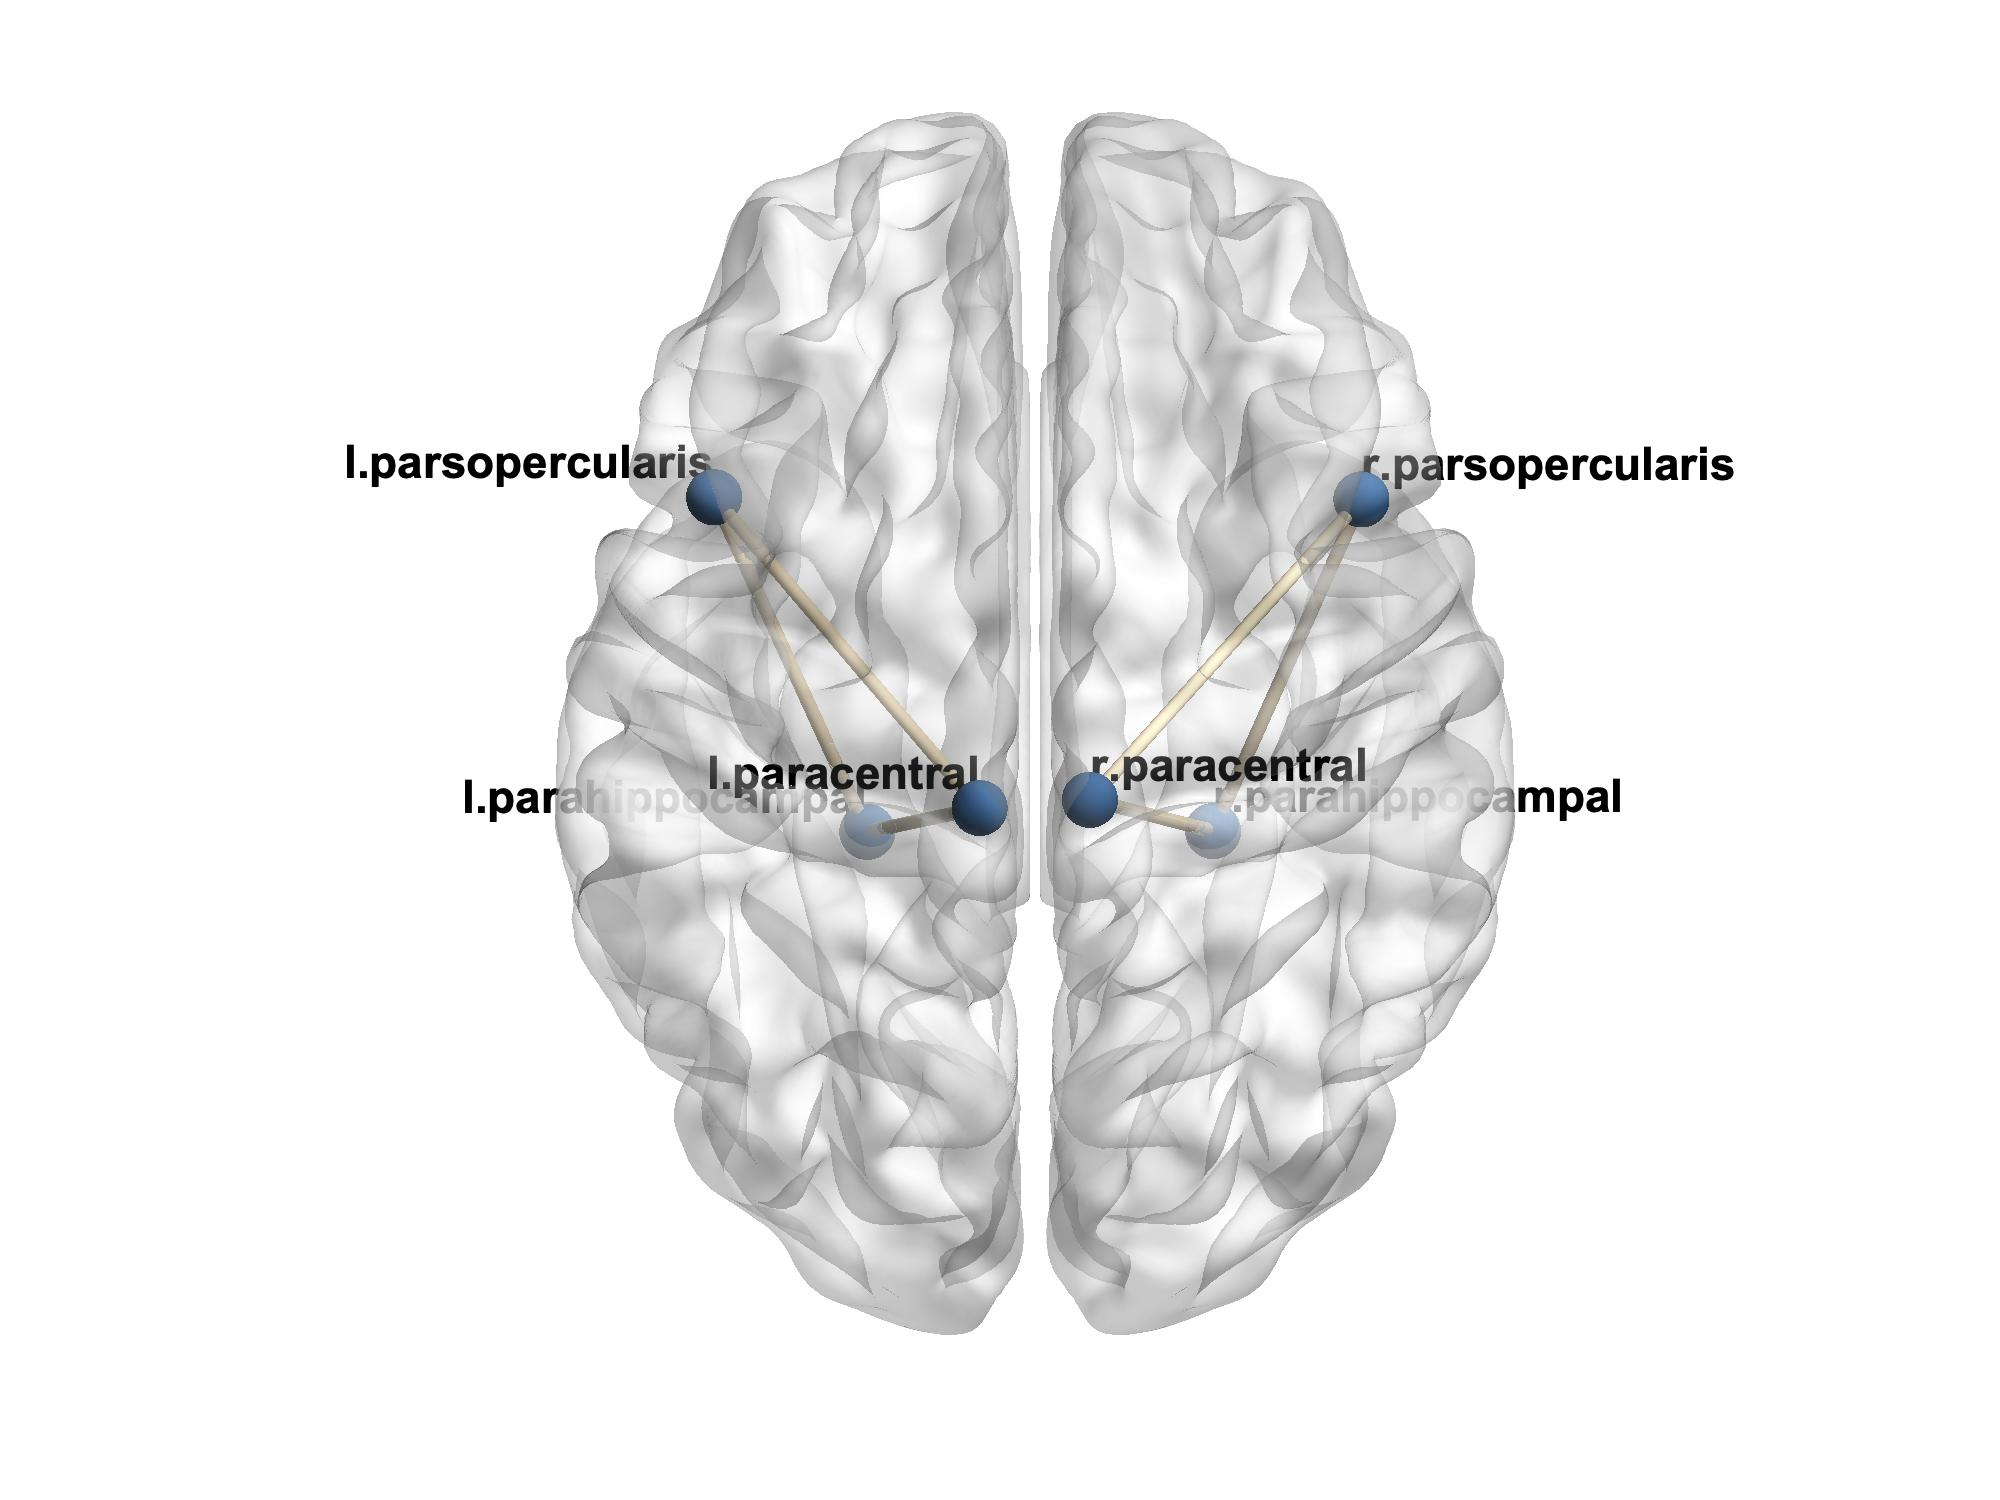
\includegraphics[width = 0.45\textwidth]{brain3.jpg}
 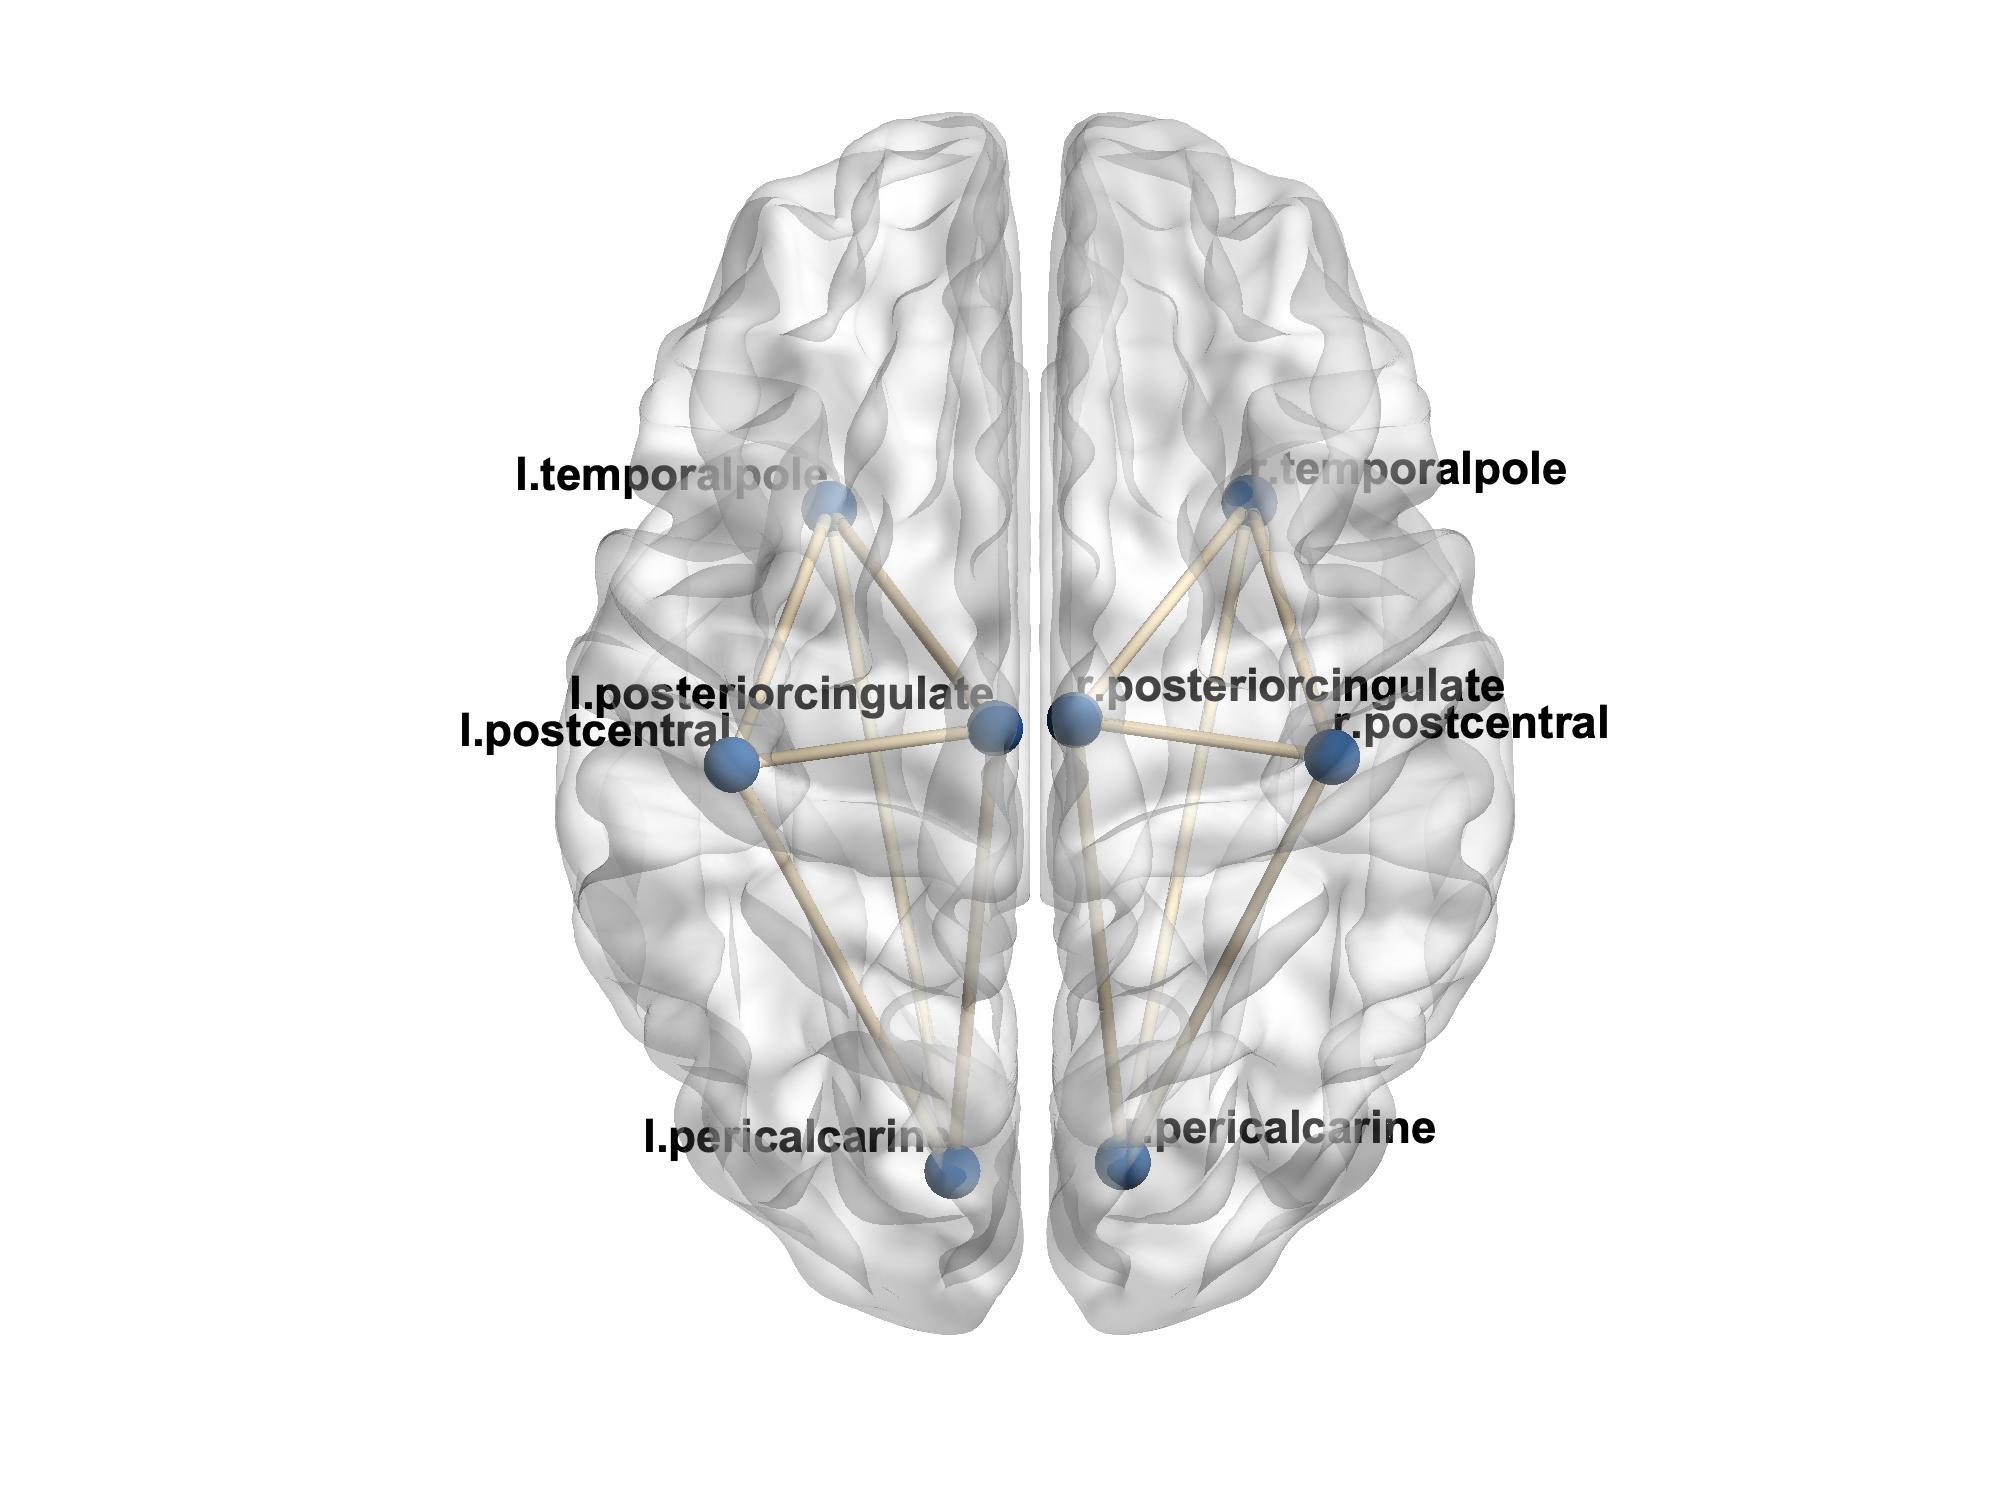
\includegraphics[width = 0.45\textwidth]{brain4.jpg}
  \label{figure:clustering}
  \caption{Brain cluster groups}
\end{figure}


\end{proof}

\bibliography{ICML.bib}
\bibliographystyle{icml2020}
\end{document}
